\section*{I.1.1.1}
Given
\[
	a = \begin{pmatrix} 1\\2\\2 \end{pmatrix}
	b = \begin{pmatrix} 3\\2\\1 \end{pmatrix}
\]
Then $a^Tb = 1*3 + 2*2 + 2*1 = 3 + 4 + 2 = 9$

\section*{I.1.1.2}
The \textit{l2-norm} or \textit{Euclidean norm} $||a|| = \sqrt{1^2 + 2^2 + 2^2} = 3$

\section*{I.1.1.3}
The outer product
\[
	ab^T = \begin{bmatrix}
		1*3 & 1*2 & 1*1 \\
		2*3 & 2*2 & 2*1 \\
		2*3 & 2*2 & 2*1
	       \end{bmatrix}
	     = \begin{bmatrix}
		3 & 2 & 1 \\
		6 & 4 & 2 \\
		6 & 4 & 2
	       \end{bmatrix}
\]

\section*{I.1.1.4}
As M is a diagonal matrix the inverse matrix of $M$ is
\[
	M^{-1} = \begin{bmatrix}
		  1/1 & 0 & 0 \\
	  	  0 & 1/4 & 0 \\
		  0 & 0 & 1/2
		 \end{bmatrix}
	       = \begin{bmatrix}
		  1 & 0 & 0 \\
	  	  0 & 0.25 & 0 \\
		  0 & 0 & 0.5
		 \end{bmatrix}
\]

\section*{I.1.1.5}
The matrix-vector product $Ma = \begin{pmatrix}
                                 1*1 + 0*2 + 0*2 \\
                                 0*1 + 4*2 + 0*2 \\
                                 0*1 + 0*2 + 2*2
                                \end{pmatrix}$
                              = $\begin{pmatrix}
                                 1 \\
                                 8 \\
                                 2
                                \end{pmatrix}$

\section*{I.1.1.6}
\[
	A^T = (ab^T)^T = \begin{bmatrix}
		          3 & 6 & 6 \\
		          2 & 4 & 4 \\
		          1 & 2 & 2
	                 \end{bmatrix}
\]

\section*{I.1.1.7}
The rank of $A = 1$, because the rows are linearly dependent. We can verify this
by observing that the first row can produce the second and third rows with a
multiple, e.g. the second row (6 4 2) is the same as the first row (3 2 1) x 2.

\section*{I.1.1.8}
As $A$ is not full rank, it is not invertible.

\section*{I.1.2.1}
The derivative of $f(w) = (wx + b)^2$ with respect to $w$ is
\begin{align*}
	((wx+b)^2)' &= (w^2 x^2 + 2wxb+b^2)' \\
	&= 2x^2w + 2xb \\
	&= 2x(xw + b)
\end{align*}

\section*{I.1.2.2}
In general
\[
	\left ( \frac{f}{g} \right )' (x) = \frac{f'(x) \cdot g(x) - f(x) \cdot g'(x)}{(g(x))^2}
\]

Therefore, differentiating for w we get:
\begin{align*}
	f(x) &= 1 \\
	f'(x) &= 0 \\
	g(x) &= (wx+b)^2 \\
	g'(x) &= 2x(wx+b) \\
	\left ( \frac{f}{g} \right )' (w) &= \frac{0 \cdot (wx+b)^2 - 1 \cdot 2x(wx+b)}{((wx+b)^2)^2} \\
	&= \frac{-1 \cdot 2x(wx+b)}{(wx+b)^4} \\
	&= \frac{-2x}{(wx+b)^3}
\end{align*}

\section*{I.1.2.3}
In general
\[
	\left ( f \cdot g \right )' (x) = f'(x) \cdot g(x) + f(x) \cdot g'(x)
\]

Therefore, differentiating for x we get:
\begin{align*}
	f(x) &= x \\
	f(x)' &= 1 \\
	g(x) &= e^x \\
	g(x)' &= e^x \\
	\left ( f \cdot g \right )' (x) &= 1e^x + xe^x
\end{align*}

\pagebreak
\section*{I.2.1}
The plots with gaussian distributions for $(\mu,\sigma)$ pairs $(-1,1)$, $(0,2)$ and
$(2,3)$ can be seen in Figure~\ref{fig:I.2.1}. The code for generating the plots
can be found in \texttt{I\_2\_1.m}, and the code for our gaussian
distribution function can be found in \texttt{unigauss.m}.

\begin{figure}[h!]
	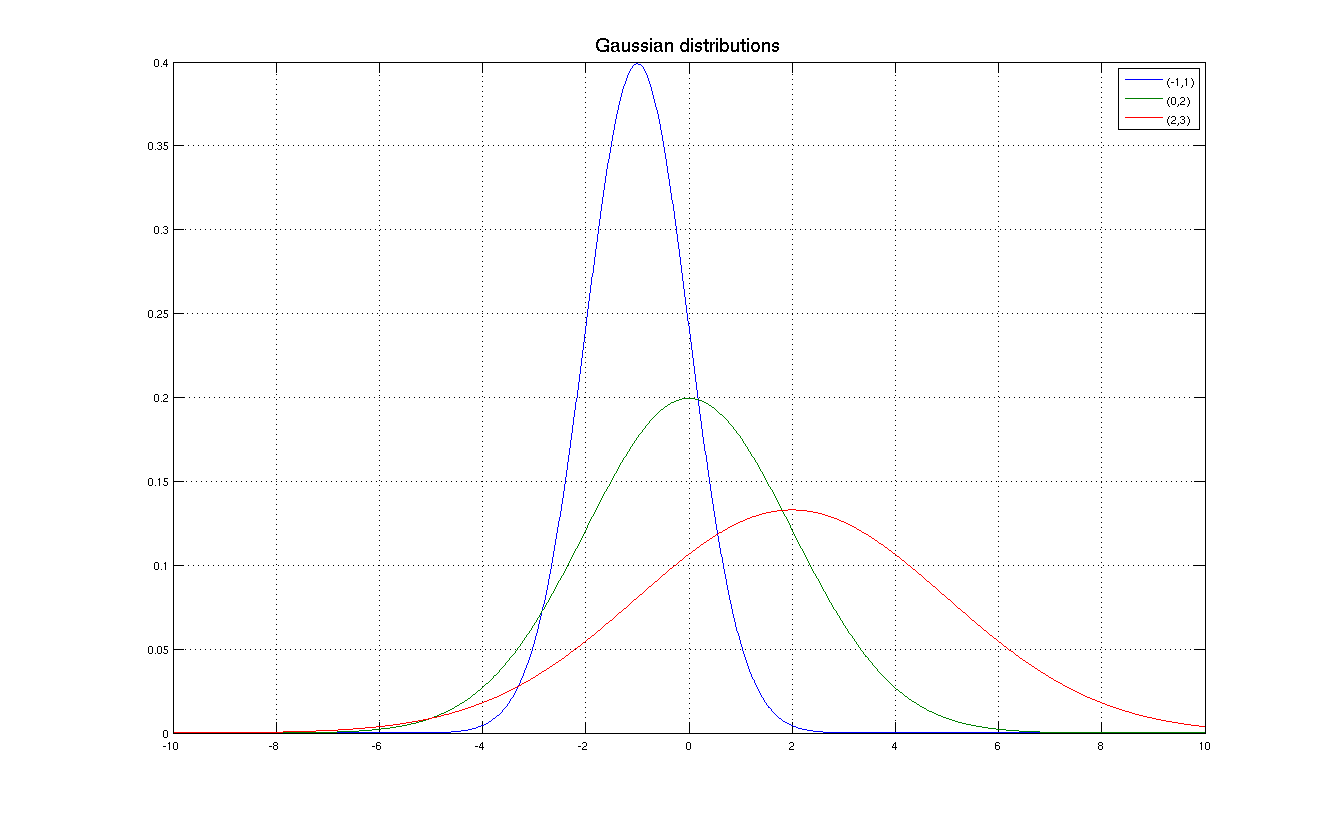
\includegraphics[width=\textwidth]{img/unigauss}
	\caption{Gaussian distributions plotted with different values for
          $(\mu, \sigma)$. \label{fig:I.2.1}}
\end{figure}

\section*{I.2.2}
Source code is available in \texttt{multigauss.m} and \texttt{I\_2\_2.m}.
Plot can be seen in Figure~\ref{fig:I.2.2}.
\begin{figure}[h!]
	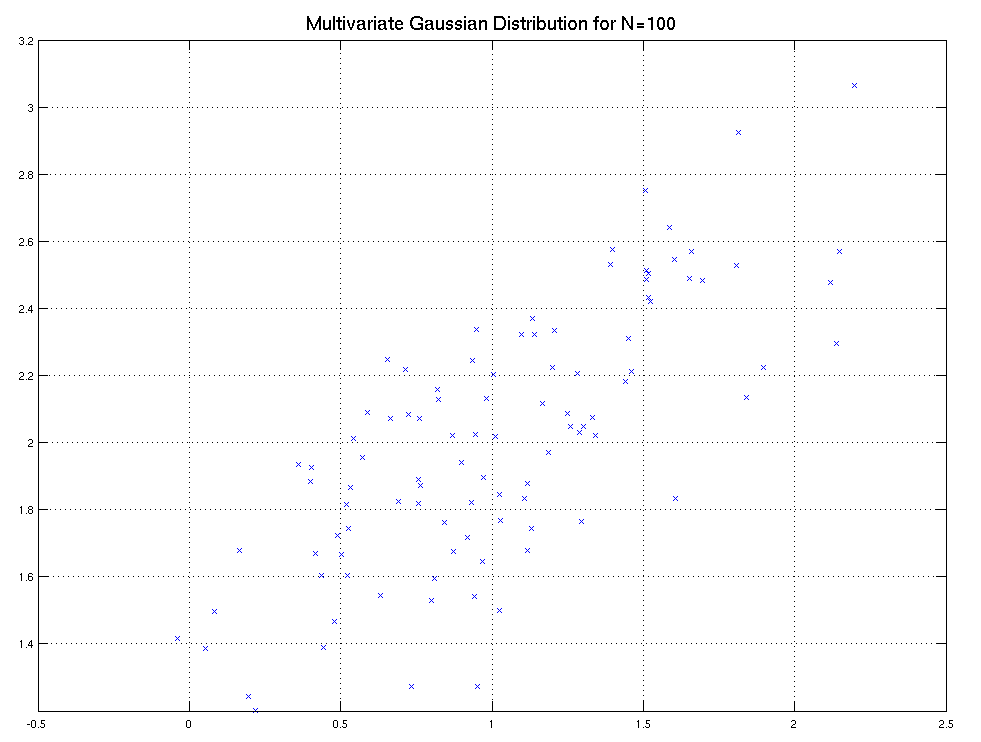
\includegraphics[width=\textwidth]{img/multigauss}
	\caption{100 points drawn from a 2-dimensional Multivariate gaussian
          distribution. \label{fig:I.2.2}}
\end{figure}

\section*{I.2.3}
The $l2$ norm of $x$ is
\begin{align*}
	mean  &= \begin{pmatrix}1 & 2\end{pmatrix}^T \\
	\mu   &= \begin{pmatrix}1.0006 & 1.9834\end{pmatrix}^T \\
	||x|| &= l2(mean - \mu) = 0.0366
\end{align*}
where $l2()$ is a function that calculates the \textit{Euclidean norm} or $l2$
norm of the vector $mean - \mu$.

Figure~\ref{fig:I.2.3} plots the points drawn along with a red circle for the
calculated mean and a green circle for $\mu$. There is a difference between the
two because the mean is calculated based on the generated data drawn from the
multivariate gaussian distribution at random. If we had a number of points
approaching infinite, the difference would approach $\overline{0}$. The source
code for this excersize can be found in \texttt{I\_2\_3.m}.

\begin{figure}[h!]
	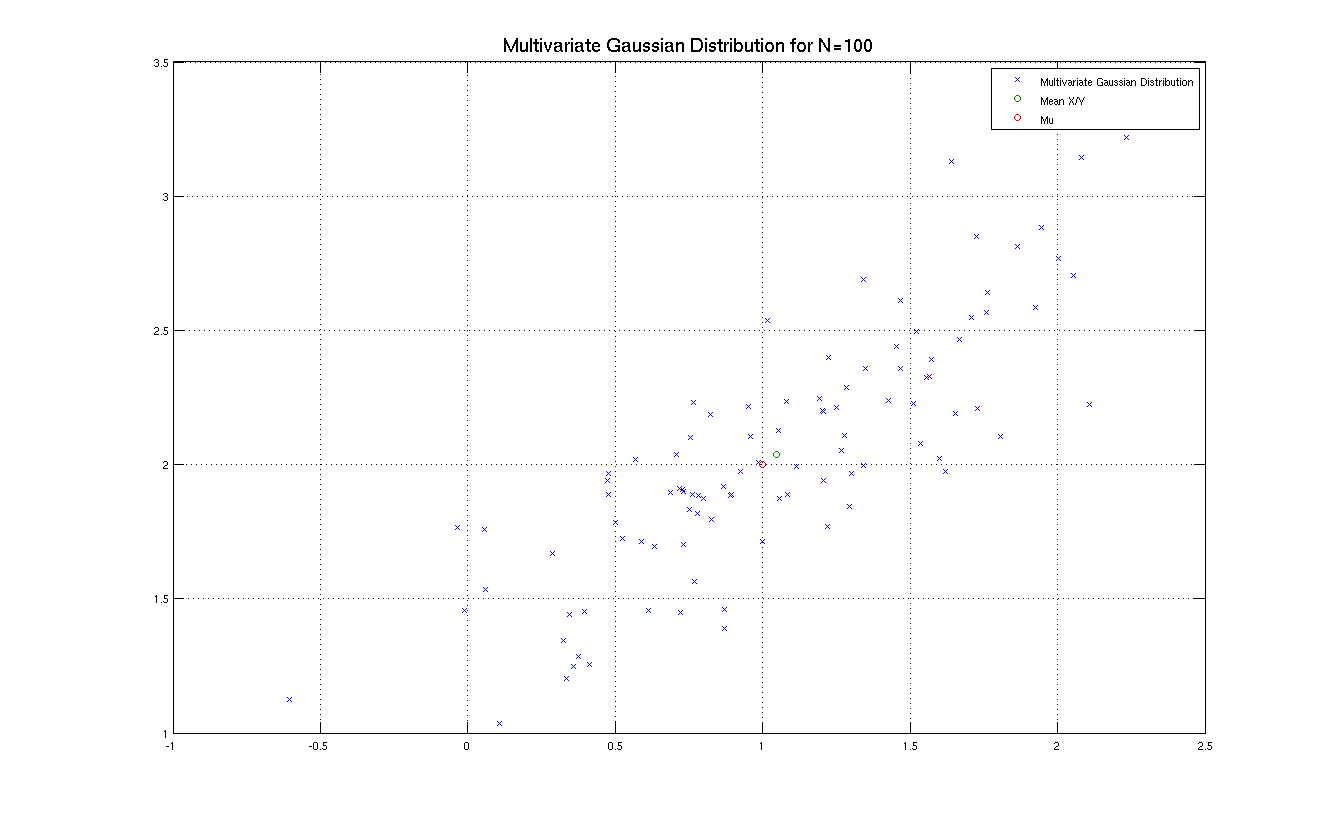
\includegraphics[width=\textwidth]{img/multigaussmeanxy}
	\caption{100 points drawn from a 2-dimensional Multivariate gaussian
          distribution, plotted with the mean of the points and of $\mu$.
        \label{fig:I.2.3}}
\end{figure}

\FloatBarrier
\section*{I.2.4}
The covariance matrix is full rank 2 and thus has two eigenvectors and
eigenvalues. Each eigenvector represents a principal component (or linearly
uncorrelated variable), and each eigenvalue a scalar representing the variance.
Intuitively, the eigenvectors form a scaled and translated coordinate system
centered at the mean of the multivariate Gaussian distribution ($\mu$). If an
eigenvalue is 0, the dimensionality is reduced by one. The larger of the two
eigenvector/value pairs represents the direction where the ellipsis is widest.
The other represents where the ellipsis is narrowest.

The covariance matrix we calculated can be found in Eq~\ref{eq:cov}.


\begin{align}
	\Sigma_{ML} &= \frac{1}{N} \sum_{n=1}^N (x_n - \mu_{ML}) (x_n - \mu_{ML})^T \notag \\
	&= \begin{pmatrix}
		0.3239 & 0.2093 \\
		0.2093 & 0.2080
	\end{pmatrix} \label{eq:cov}
\end{align}

Figure~\ref{fig:I.2.4.1} shows a plot of the Multivariate gaussian distribution,
plotted with the mean, $\mu$ and the two eigenvectors centered in the
distribution $\mu$. Figure~\ref{fig:I.2.4.1.rot} shows a plot of the 3 rotated
distributions along with the distribution rotated to match the largest
eigenvector along the x-axis. The angle needed for this was $-37.2564^o$ in our
case. Source code is available in \texttt{multigauss.m} and \texttt{I\_2\_4.m}.
The angle is calculated by by the formula
\[-\text{arctan}(\text{eig}(\Sigma_{\text{ML}}))\] which return the angle needed
for rotating the distribution so its eigen vector is parallel to the x-axis.


\begin{figure}[h!]
	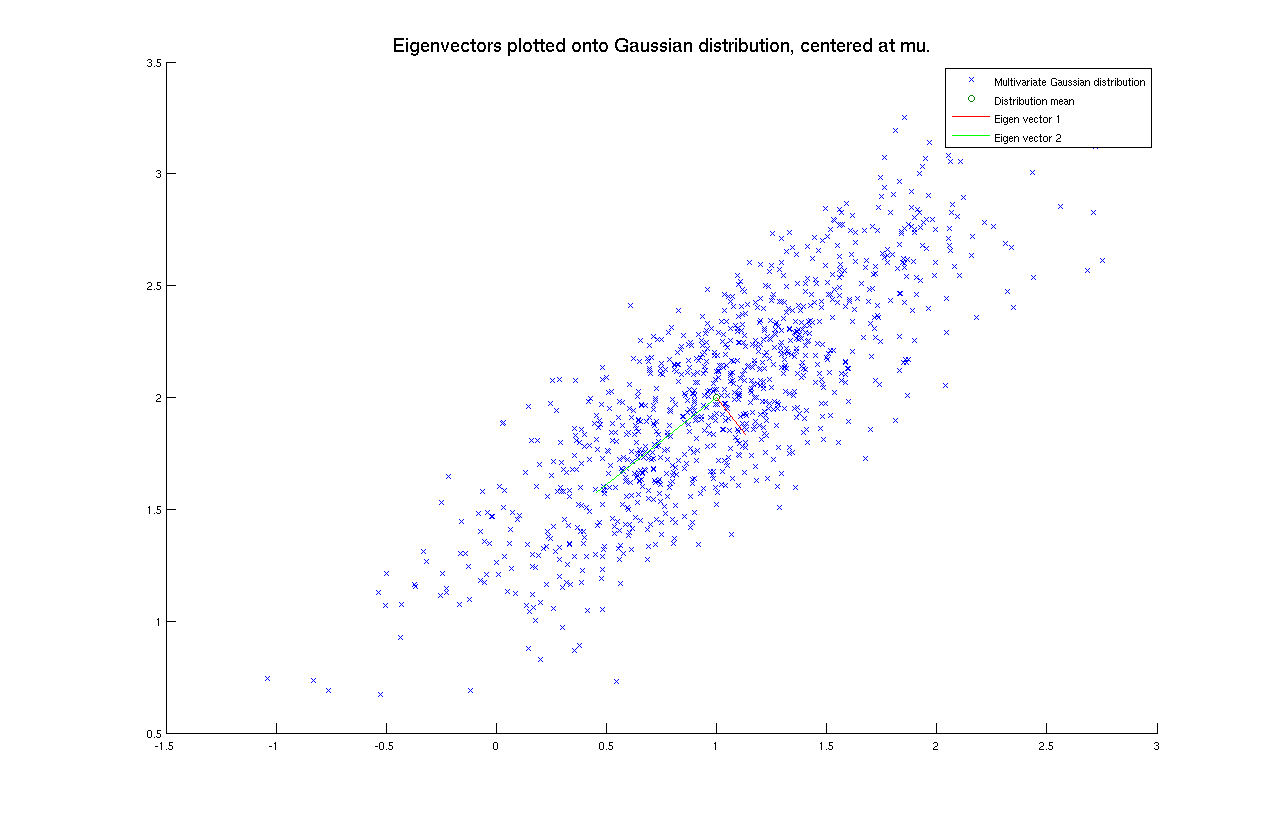
\includegraphics[width=\textwidth]{img/multigausseigen}
	\caption{100 points drawn from a 2-dimensional Multivariate gaussian
          distribution, plotted with the mean of the distribution, the value of
          $\mu$ and the two eigenvectors centered in the distribution
          $\mu$. \label{fig:I.2.4.1}}
\end{figure}

\begin{figure}[h!]
	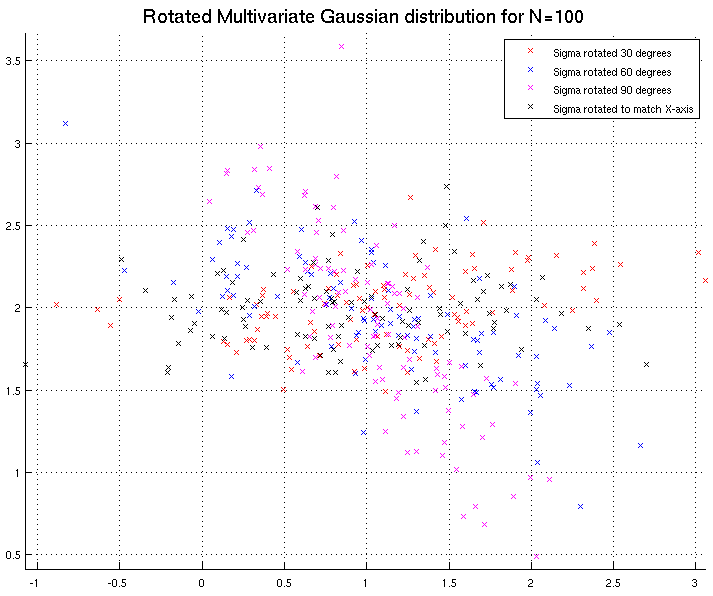
\includegraphics[width=\textwidth]{img/multigaussrotate}
	\caption{100 points drawn from a 2-dimensional Multivariate gaussian
          distribution, rotated at 30, 60 and 90 degrees and lastly also aligned
          along the x-axis, all distributions in their own
          color. \label{fig:I.2.4.1.rot}}
\end{figure}

\FloatBarrier
\pagebreak
\section*{I.3}

Given:

\begin{align*}
	\mu = \begin{pmatrix}
		\mu_a \\
		\mu_b \\
		\mu_c
	\end{pmatrix} \quad
	x = \begin{pmatrix}
		x_a \\
		x_b \\
		x_c
	\end{pmatrix} \quad
	\Sigma = \begin{bmatrix}
		\Sigma_{aa} & \Sigma_{ab} & \Sigma_{ac} \\
		\Sigma_{ba} & \Sigma_{bb} & \Sigma_{bc} \\
		\Sigma_{ca} & \Sigma_{cb} & \Sigma_{cc}
	\end{bmatrix}
\end{align*}

We wish to discover an expression for the conditional distribution $p(x_a|x_b)$
in which $x_c$ has been marginalized out.

We now use, that a vector of length $i$ and a vector of length $j$
can be seen as a vector of length $k=i+j$, and similarly with matrices.

Let:

\begin{align*}
	\mu = \begin{pmatrix}
		\mu_d \\
		\mu_c
	\end{pmatrix} \quad
	x = \begin{pmatrix}
		x_d \\
		x_c
	\end{pmatrix} \quad
	\Sigma = \begin{bmatrix}
		\Sigma_{dd} & \Sigma_{dc} \\
		\Sigma_{dc} & \Sigma_{cc}
	\end{bmatrix}
\end{align*}

now we have from chapter 2.3.2 that:

\begin{align*}
	\mathbb{E}[x_d] &= \Sigma_{dd} \\
	&= \begin{bmatrix}
		\Sigma_{aa} & \Sigma_{ab} \\
		\Sigma_{ba} & \Sigma_{bb}
	   \end{bmatrix} \\
	\text{cov}[x_d] &= \mu_d \\
	&= \begin{pmatrix}
		\mu_a \\
		\mu_b
	   \end{pmatrix}
\end{align*}

when $x_c$ has been marginalized out.

Now we have from chapter 2.3.1 for the conditional distribution $p(x_a | x_b)$:

\begin{align*}
	\mu_{a|b} &= \mu_a + \Sigma_{ab} \Sigma_{bb}^{-1}(x_b - \mu_b)
	\Sigma_{a|b} &= \Sigma_{aa} - \Sigma_{ab} \Sigma_{bb}^{-1} \Sigma_{ba}.
\end{align*}

\pagebreak
\section{I.4}
\subsection{I.4.1}
The result of our KNN implementation for different k-values and datasets is
shown in Table \ref{tab:knn-res}. The code to run this particular experiment
is in \texttt{I\_4\_1.m}.
\begin{table}
\center
\begin{tabular}{|l|l|l|}
\hline
Description          & $K$-value & Accuracy in \% \\\hline
Run on training data & 1         & $100  \%$ \\
Run on test data     & 1         & $81.5 \%$ \\
Run on training data & 3         & $86.0 \%$ \\
Run on test data     & 3         & $81.5 \%$ \\
Run on training data & 5         & $83.0 \%$ \\
Run on test data     & 5         & $68.4 \%$ \\\hline
\end{tabular}
\caption{The results from I.4}
\label{tab:knn-res}
\end{table}

With $K=1$ and running against the training set, the accuracy is 100\% since any
entry will be matched against itself, and only itself. We also see a general
loss of accuracy as $K$ increases. This may be because the point gets matched up
against a larger and larger set of the total points, and if there is inherent density
clusters in the data then we risk going further and further out as K increases.

\subsection{I.4.2}
The code for this experiment is in \texttt{I\_4\_2.m}. It uses several auxiliary
files found in the same directory. Given a set of possible k values `PossibleKValues'
the following pseudocode runs cross-validation to find the average loss experienced amongst
each of the five folds of a cross-validation for each given $k$ value, and then selects the
best $k$ as the one with the lowest average loss:

\begin{algorithmic}
	\For{$k$ in PossibleKValues}
		\State $\text{subsets} \gets \text{shuffleSplit(dataset,5)}$
		\For{$cv = 1\ to\ 5$}
			\State $\text{test} \gets \text{subsets}[cv]$ \Comment{bucketJoiner function}
			\State $\text{train} \gets \text{subsets} - \text{test}$ \Comment{bucketJoiner function}
			\State $\text{pred} \gets \text{kNN(k, train.X, train.y, test.X)}$
			\State $\text{loss}[cv] \gets 1 - \frac{pred - test.y}{\text{length(pred)}}$
		\EndFor
		\State $\text{avgLoss}[k] \gets \text{mean(loss)}$
	\EndFor
	\State $\text{bestK} \gets \text{min(avgLoss)}$ \Comment{k for which avgLoss is lowest.}
\end{algorithmic}

The \texttt{shuffleSplit} method splits a dataset into $n$ randomized disjoint
subsets, in this case $n = 5$. The \texttt{bucketJoiner} method joins one or
more of these disjoint subsets into a single, larger subset by appending one
onto the other. The $k$-value with the lowest average loss for our data was
$5$, with an accuracy of approximately $80\%$. The accuracy on the test data is
$68,4\%$.

\subsection{I.4.3}
The code for this experiment can be found in \texttt{I\_4\_3.m}. The experiment
is very similar to that of \texttt{I.4.2}. Before cross-validating, we normalize
the data using the method found in \texttt{scale.m}.

The $\mu$ values for the training data is $(5.7560, 0.3017)$ and $\sigma^2 =
(0.6958, 0.0018)$. Normalizing the training data gives $\mu = (-0.3466*1^{-14},
-0.1823*1^{-14})$ and $\sigma^2 = (1.0000, 1.0000)$. After the normalization of
the test data with the values found for the training data the test data have
$\mu = (0.2073, 0.43)$ and $\sigma^2 = (1.0914, 1.2732)$. Running the test from
\texttt{I.4.2} now gives $K_{\text{best}}=1$ and an accuracy of $78,95\%$ on the
test data, and $100\%$ accuracy on the training data. The last result is
expected since when $K=1$ any entry will be closest to itself (the euclidian
distance is 0.)

%The $(\text{mean},\text{var})$ of the training data is: $(3.0288,7.8218)$, the
%test data after the normalization have the values $(0.1545,1.0000)$. The most
%optimal $K$ value is still 5, but the accuracy has increased to $71,05\%$ when
%using the normalized test set.
